\chapter{Plotting}
\index{plotting}
\label{c:plotting}

\begin{figure}[tb]
  \centering
  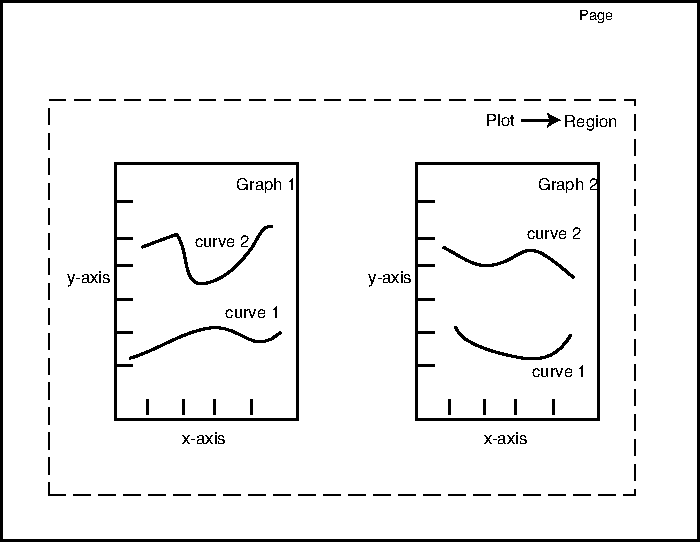
\includegraphics{plot.pdf}
  \caption[A plot has a collection of graphs.]
{A plot has a collection of graphs and a graph has a 
collection of curves. A plot becomes visible when it is associated
with some region on the page using the \vn{place} command. Note that
on the actual page the plot/region border is not visible.}
  \label{f:plot}
\end{figure}

Some definitions:
  \vspace*{-3ex}
\begin{description}
\index{curve|hyperbf}
\item[Curve] \Newline
A \vn{curve} is a set of (x,y) points to be plotted.
\index{graph|hyperbf}
\item[Graph] \Newline
A \vn{graph} consists of horizontal and vertical axes along with a set
of \vn{curve}s that are plotted within the graph. 
\index{plot|hyperbf}
\item[Plot] \Newline
A \vn{plot} is essentially a collection of \vn{graphs}.
\index{page|hyperbf}
\item[Page] \Newline
The \vn{page} refers to the X11 window where graphics are displayed or the 
corresponding printed graphics page.
\index{region}
\item[Region] \Newline
The \vn{page} is divided up into a number of rectangles called
\vn{regions}. \vn{Regions} may overlap.
\end{description}

\index{template plot}\index{region}\index{place command}
\index{plot!initialization file}
The plot initialization file (cf.~Chapter~\ref{c:init}) defines a set of \vn{template
plots}. A \vn{template} defines what type of data is to be plotted (orbit, beta function,
etc.), how many \vn{graphs} there are, what the scales are for the \vn{graph} axes, how
the \vn{graph}s are laid out, etc.  The plot initialization file also defines a set of
\vn{region}s within the \vn{page}. Any \vn{template plot} can be placed in any
region. Using the \vn{place} command (see Chapter~\ref{c:command} for a full descriptions
of all commands) one can assign a particular \vn{template plot} to a particular region for
plotting.  The relationship between \vn{region}, \vn{plot}, \vn{graph}, and \vn{curve} is
shown graphically in Figure~\ref{f:plot}.

Figures~\ref{f:plot.page1} and \ref{f:plot.page2} show examples of a plot
\vn{page}. Figure~\ref{f:plot.page1} was generated by defining two regions called \vn{top}
and \vn{bottom} in the plot initialization file. The \vn{top} region was defined to cover
the upper half of the \vn{page} and the \vn{bottom} region was defined to cover the bottom
half. \vn{Template plots} were defined to plot phase and orbit data from a defined set of
detector elements in the lattice. Each \vn{template plot} defined two graphs which in both
cases where assigned the names \vn{x} and \vn{y}. The orbit \vn{template plot} was placed
in the \vn{top} region and the phase \vn{template plot} was placed in the \vn{bottom}
region. The horizontal axis numbering is by detector \vn{index}.  Displayed plots are
referred to by the \vn{region} name (\vn{top} and \vn{bottom} in this case). Individual
graphs and curves are referred to using the nomenclature \vn{region.graph.curve}. Thus, in
this example, the horizontal orbit graph would be referred to as \vn{top.x}.  Using the
\vn{set plot}, \vn{set graph}, or \vn{set curve} commands (\sref{s:set}) one can then
specify what \vn{components} are plotted. ``\vn{component}'' refers to \vn{measured},
\vn{reference}, \vn{model}, \vn{base}, and/or \vn{design} data (\sref{s:plot.data}).
Notice that the same \vn{template plot} can be assigned to different \vn{regions} and the
plots in different \vn{regions} can have different scales for their axes or different
\vn{components}. In the example in Figure~\ref{f:plot.page1}, the \vn{component} for the
\vn{top} plot is \vn{model} and for the \vn{bottom} plot it is \vn{model - design}.

Plots may be referred to by their template name or by the name of the region they are
placed in. For example, the orbit plot in Figure~\ref{f:plot.page1} may be referred to
using the region name (\vn{top}) or the template name (\vn{orbit}). A template may be
placed in multiple regions.  For example, you may wish to plot the \vn{model} data for the
orbit in one region and the \vn{design} data for the orbit in another region. In this case
the command \vn{scale orbit} would scale the plots in both regions while to scale the plot
in only one of the regions you would need to use the region name.

A graph of a plot is specified using the format \vn{plot_name.graph_name} where
\vn{plot_name} is a template or region name and \vn{graph_name} is the name of the
graph. For example, if the horizontal orbit graph of the \vn{orbit} plot is named \vn{x}
then it would be referred to as \vn{orbit.x} or \vn{top.x}. If a plot has only one graph,
the graph may be specified by just using the plot name.

A curve within a graph is specified using the format
\vn{plot_name.graph_name.curve_name}. If a graph has only one curve, the curve may be
specified using only the graph name \vn{plot_name.graph_name}. Additionally, if the there
is only one curve in a plot, the curve can be specified by just using the \vn{plot_name}.

The \vn{use}, \vn{veto}, \vn{restore}, and \vn{clip} commands are used to control what
data is used in fitting the model to the data in the optimization process (see
Chapter~\ref{c:opti}). The general rule is that these commands only affect measured and
reference data. If plotting \vn{model}, \vn{design} and/or \vn{base} data then the data
will be displayed irregardless. If plotting \vn{meas} and/or \vn{ref} data then the data
displayed will vary with these commands.  \vn{meas} or \vn{ref} data vetoed for display is
also vetoed for fitting.  However, measured data that is off the vertical or horizontal
scale may still be used by the optimizer unless vetoed with the \vn{veto} or \vn{clip}
command.  If there are data points off the vertical scale then ``**Limited**'' will appear
in the upper right-hand corner of the graph. If plotting measured data then these points
off scale will still be used by the optimizer.

The \vn{x_axis} and \vn{x_scale} commands are used to set the axis type and scale for each
graph. The axis type can be either \vn{index}, \vn{ele_index} or \vn{s} which corresponds
to the data index number, element index number and longitudinal position in the lattice
(from element 0) respectively.

Figure~\ref{f:plot.page2} shows another example of a plot \vn{page}.  In this case the
\vn{page} was generated by again defining two vertically stacked regions but in this case
the regions have different heights.  A \vn{template plot} with a single graph was placed
in the bottom most \vn{region}.  This \vn{graph} contains a \vn{key_table}.  A
\vn{key_table} is used in conjunction with \vn{single mode} and is explained in
Chapter~\sref{c:single}. A \vn{template plot} containing five \vn{graphs} was placed in
the uppermost region. The uppermost \vn{graph} of this \vn{template plot} contains a
\vn{lat_layout} which shows the placement of lattice elements.  What elements are
displayed in a \vn{lat_layout} and what shapes they are represented by is specified in the
initialization file. The horizontal scale is longitudinal position (\vn{s}).  The
remaining four graphs show dispersion and beta data from two different universes
representing the low energy and high energy transport in an energy recovery linac. The
individual data points here (hard to see in this example) have been slaved to the
\vn{lat_layout} and represent the beta and dispersion at the edges of the displayed
elements in the \vn{lat_layout}.

\begin{figure}
  \centering
  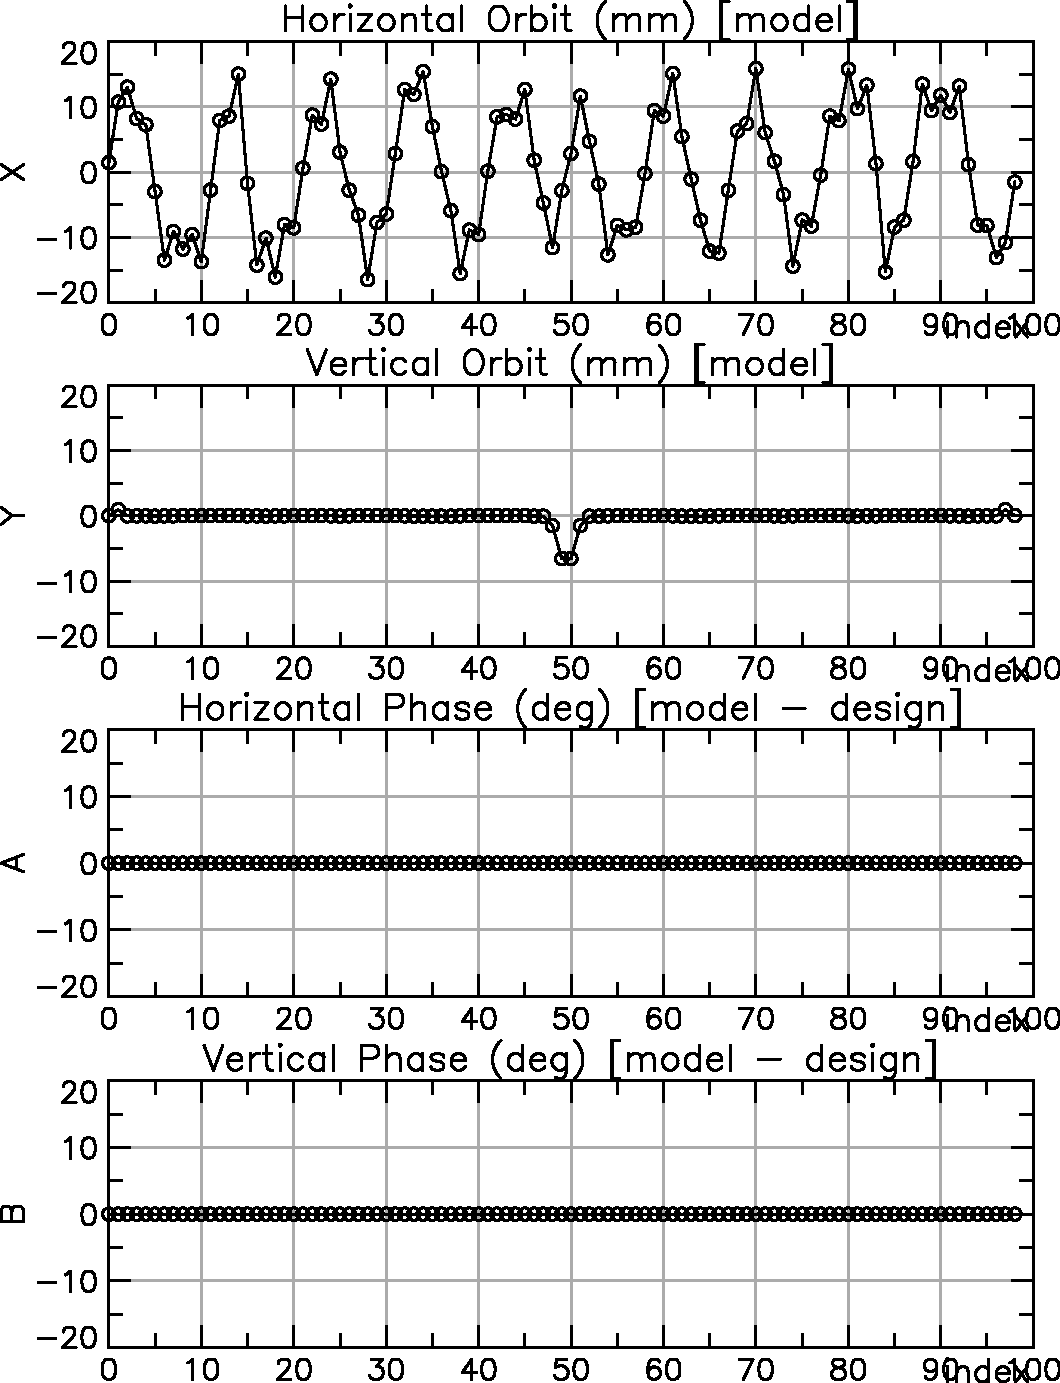
\includegraphics[width=5in]{plot-page1.pdf}
  \caption{Example of a plot page}
  \label{f:plot.page1}
\end{figure}

\begin{figure}
  \centering
  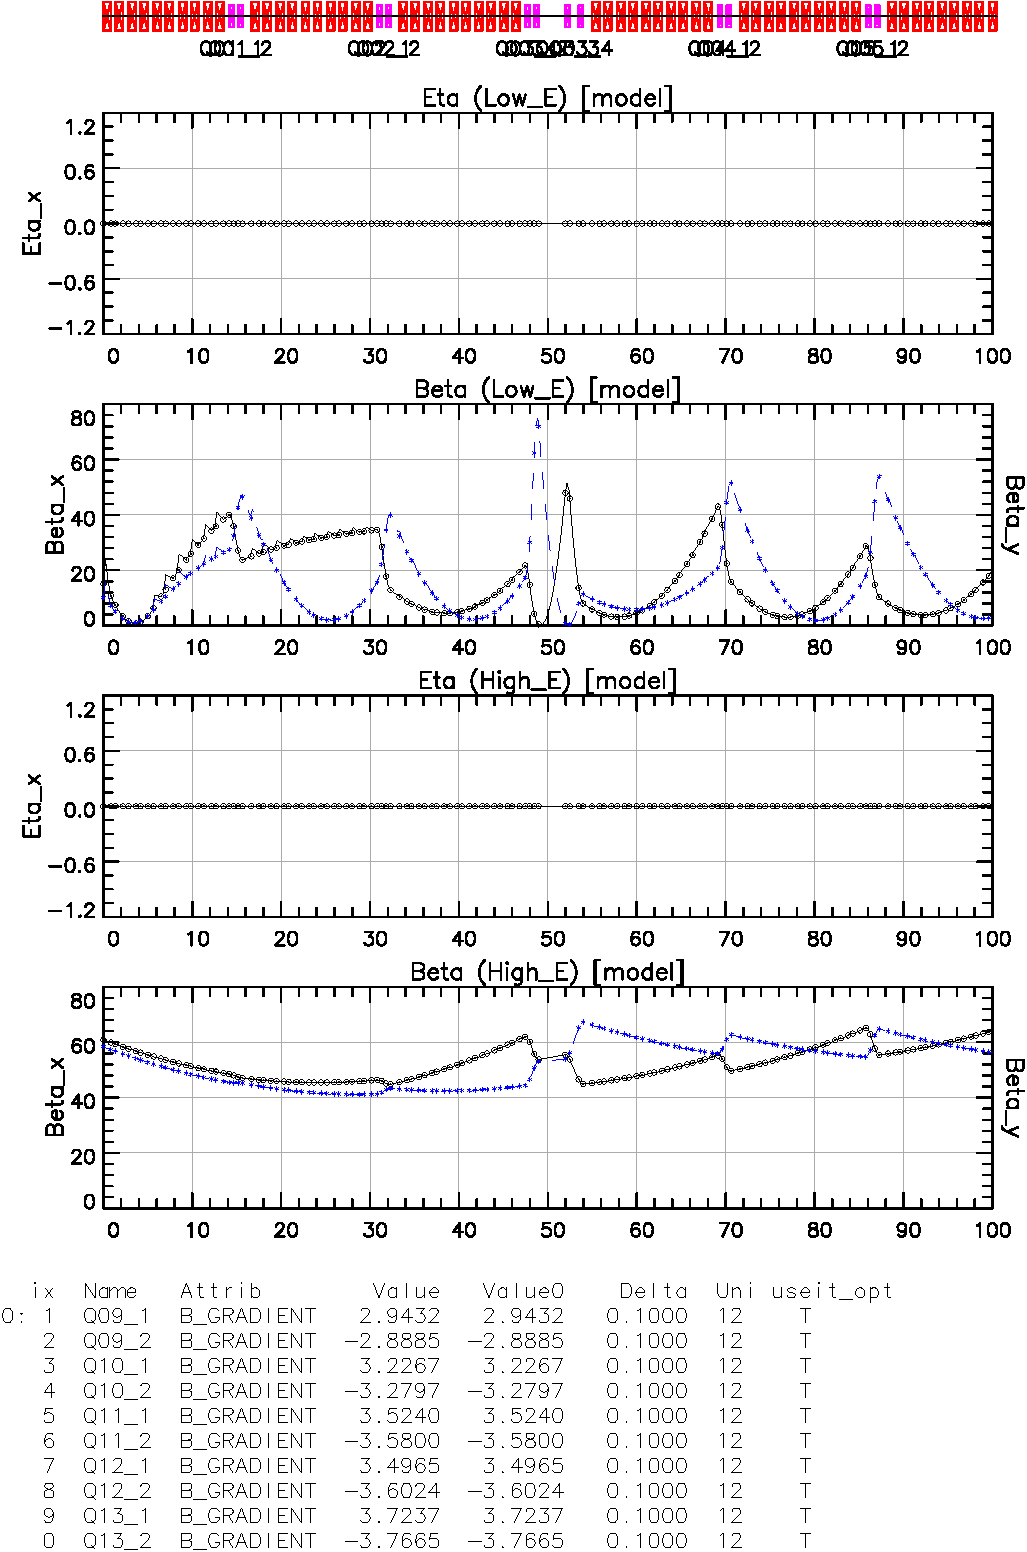
\includegraphics[width=5in]{plot-page2.pdf}
  \caption{Another example of a plot page.}
  \label{f:plot.page2}
\end{figure}

\vfill
\break
